\documentclass[11pt,a4paper]{article}

\usepackage{fullpage}
\usepackage{hyperref}
\usepackage{graphicx}
\usepackage{float}

\usepackage{fancyhdr}
\pagestyle{fancy}
\fancyhf{}
\usepackage{todonotes}                %% notes from the authors

\renewcommand{\headrulewidth}{0pt}
\renewcommand{\footrulewidth}{0pt}

\newcommand*{\escape}[1]{\texttt{\textbackslash#1}}

\fancypagestyle{firstpagefooter} {
	\lfoot{\tiny{Version: 25.09.2018}}
	\cfoot{}
	\rfoot{\thepage}
	
}

\lfoot{Name: Mohammed Ajil Legi: 11-948-734}
\rfoot{\thepage}

\begin{document}

\title{Advanced Systems Lab Report\\ \normalsize{Autumn Semester 2018}}
\author{Name: Mohammed Ajil\\Legi: 11-948-734}
\date{
	\vspace{4cm}
	\textbf{Grading} \\
	\vspace{0.5cm}
	\begin{tabular}{|c|c|}
		\hline  \textbf{Section} & \textbf{Points} \\
		\hline  1                &                 \\ 
		\hline  2                &                 \\ 
		\hline  3                &                 \\ 
		\hline  4                &                 \\ 
		\hline  5                &                 \\ 
		\hline  6                &                 \\ 
		\hline  7                &                 \\ 
		\hline \hline Total      &                 \\
		\hline 
	\end{tabular} 
}
\maketitle
\thispagestyle{firstpagefooter}

\newpage
\listoftodos
\newpage

\section{System Overview (75 pts)}
%
\subsection{Class Overview}
%
\begin{figure}[H]
    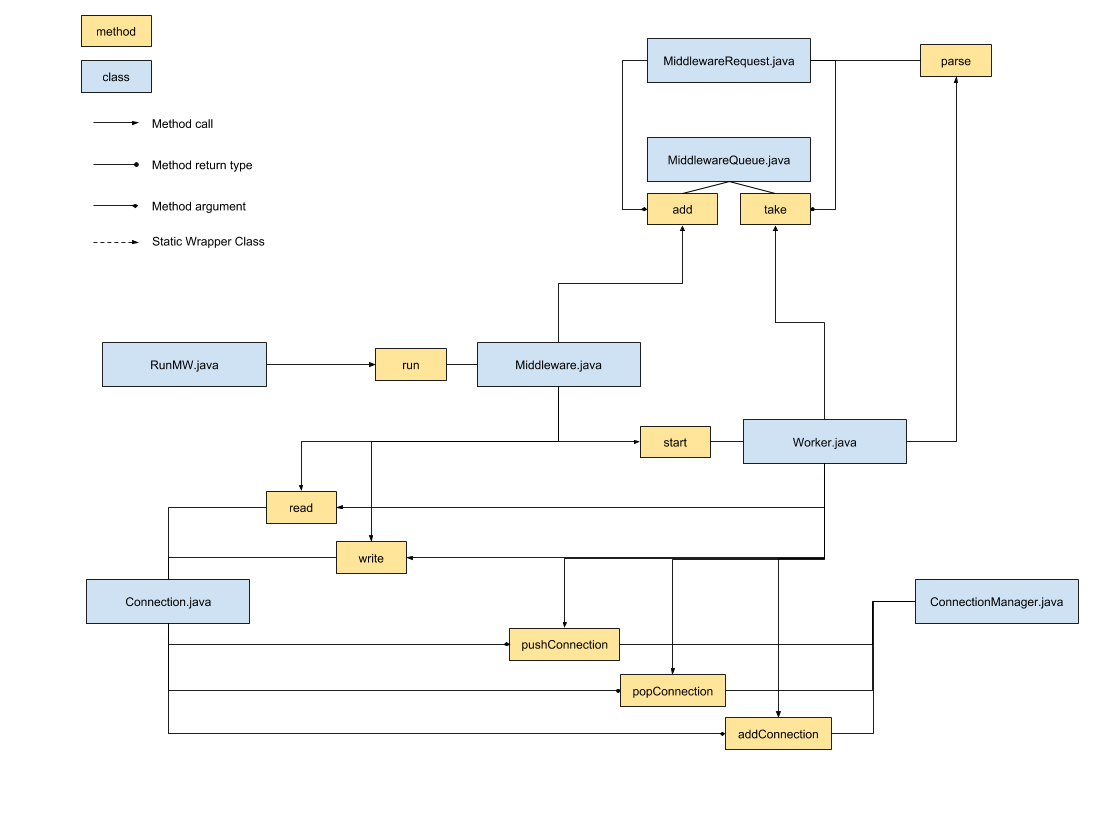
\includegraphics[width=\linewidth]{../illustrations/class_diagram.png}
    \caption{Class Diagram}
    \label{fig:class_diagram}
\end{figure}
%
We will start by looking at a class diagram of the middleware.
%
In \ref{fig:class_diagram} we can see all the classes that compose the middleware.
%
The system is represented in its running state, i.e. all methods that are only used when starting up are omitted.
%
In the following paragraphs we will look at each of the components in detail.
%
\paragraph{\texttt{RunMW.java}}
%
This class has a single responsibility. It parses the command line arguments and runs the middleware thread using these.
%
\paragraph{\texttt{MiddlewareRequest.java}}
%
This class represents a request coming from a client.
%
The object holds all the relevant data of the request, i.e. all time measurements, whether or not the request was successful and the \texttt{Connection} object of the client that sent the request.
%
In this class we implement the parsing method, that scans the command string and populates fields in the object.
%
If the middleware is running in sharded mode, \texttt{MULTI-GET} requests will be sharded into a list of commands.
%
\paragraph{\texttt{Middleware.java}}
%
This class represents the net thread of the system. Its responsibilities are first to accept client connections and register them so that we can start accepting requests. 
%
Second the thread also reads requests from already acccepted client connections and enqueues them in the \texttt{MiddlewareQueue}.
%
To avoid busy waiting and accessing client sockets that do not have data to read we use a \texttt{Selector}. 
%
Basically this is a mechanism that allows us to register connections and the selector will deliver only the connections that have data ready to read.
%
We also register the server socket with the selector and receive connections that are ready to be accepted.
%
Using this we can maximize the utilization of the CPU time used by the net thread.
%
We will look at the process of accepting connections and requests in detail in section~\ref{subsec:handlingRequests}
%
\paragraph{\texttt{MiddlewareQueue.java}}
%
In this middleware the \texttt{MiddlewareQueue} is a first class citizen, as are the workers and the net thread.
%
This decision is made based on the fact that the queue should not be owned by either the net or the worker threads.
%
The queue is not much more than a static wrapper around a \texttt{BlockingQueue}.
%
The access to take a request out of the queue is synchronized, so that we avoid processing the same request twice.
%
\paragraph{\texttt{Worker.java}}
%
In this class the actual processing of the request is done.
%
Depending on the type of the request that worker threads handle them differently. 
%
This will be adressed in detail in section~\ref{subsec:handlingRequests}.
%
In general a worker thread takes a request out of the \texttt{MiddlewareQueue}, after that the worker calls the parse method offered by \texttt{MiddlewareRequest}.
%
After that several new fields in the request object are populated, such as \texttt{RequestType} for example.
%
The parsed request will then be scheduled on the memcached servers depending on the server mode and request type.
%
The worker then waits for the responses from the memcached servers, parses the responses and then sends the appropriate response to the client.
%
After finishing processing the request the worker will then log the relevant fields for the analysis in a CSV format.
%
\paragraph{\texttt{Connection.java}}
%
The connection class is a convenience wrapper around a \texttt{SocketChannel}.
%
It represents both the client and server connections.
%
It allows us to specify if a connection should be blocking or not.
%
The goal of this class is that when using a connection we do not need to care about the configuration and how to read from the socket, instead we can just call the \texttt{read()} method and the different modes are handled internally.
%
\paragraph{\texttt{ServerManager.java}}
%
This class is used by the worker threads.
%
The \texttt{ServerManager} holds the \texttt{Connection} objects for the memcached servers.
%
This class offers the method \texttt{getConnection(int i)}, which will return the appropriate server connection based on the integer that is passed, such that the load is scheduled in a round robin fashion.
%
We will see in section~\ref{subsec:handlingRequests} how exactly that is handled based on the Id of the request.
%
Even if the request will go to all memcached servers it still makes sense to choose the first server to send the request to based on round robin.
%
This distributes the load even if we only have Set requests.
%
\subsection{Message Parsing}
%
As mentioned before the first thing the workers do with the request is parse it.
%
Parsing means mainly two things here, first we will determine the type of request we are looking, this tells us how to further handle the request.
%
Second, if applicable, we set the \texttt{MULTI-GET} Size.
%
In the specific case of running the server in sharded mode and receiving a \texttt{MULTI-GET} Request we will split the keys in the request and depending on the \texttt{MULTI-GET} Size and number of servers populate a list of commands, this is known as "sharding" a command.
%
The number of shards is exactly \texttt{min(multiGetSize, numServers)}
%
\subsection{Response Parsing}
%
In two cases, specifically when handling sharded \texttt{MULTI-GET} or \texttt{SET} requests we need to do some work before sending the request to the client.
%
\\
%
In the case of \texttt{SET} requests we need to make sure that the key was set on all the three servers.
%
That can be achieved by simply checking if all the responses equal \texttt{STORED\escape{r}\escape{n}}.
%
If that is the case we send the same response back to the client.
%
If not, it does not matter if we receive an error or if the key was simply not stored on some or all servers, we respond to the client with \texttt{NOT STORED\escape{r}\escape{n}} to let the client know that it should retry setting the key.
%
\\
%
In the case of sharded \texttt{MULTI-GET} requests we need to combine the responses from all servers back to a single response and send it back to the client.
%
This is done by simply removing the end marker from all responses, concatenating them and then adding the end marker back at the end.
%
Finally we count the keys and record how many keys we have received to be able to calculate the miss rate and then we send the response on its way to the client.
%
\subsection{Logs}
%
To handle the logs in this multithreaded setting we use \texttt{log4j}.
%
The logs from all the workers are consolidated into a single CSV file per middleware, this is handled by \texttt{log4j}.
%
After finishing processing a request the workers will call the \texttt{toString()} method implemented by the \texttt{MiddlewareRequest} to produce a CSV log line.
%
This log line is passed to \texttt{log4j}.
%
\subsection{Queues}
%
\begin{figure}[H]
    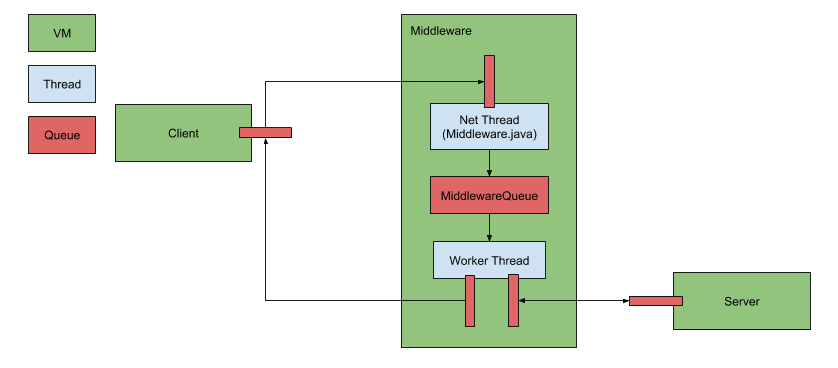
\includegraphics[width=\linewidth]{../illustrations/threads_and_queues.png}
    \caption{Threads and Queues}
    \label{fig:threads_and_queues}
\end{figure}
%
In figure~\ref{fig:threads_and_queues} we can see an illustration of threads and queues in the system.
%
The arrow directions indicate the flow of requests.
%
Arrows connecting different VMs represent sockets, thus the all queues except the MiddlewareQueue refer to socket queues.
%
The illustration only shows one instance of a client, a server, and a worker thread.
%
In the full system there are three instances of clients and servers.
%
Depending on the configuration there are also many worker threads.
%
The queues and connections for these variable components are also replicated for the number of instances.
%
\subsection{Handling Requests}\label{subsec:handlingRequests}
%
In this section we go into detail on how the middleware handles incoming connections and how the different types of requests are handled by the middleware.
%
What follows are sequence diagrams that model the behaviour of the system for different request types.
%
Important to note here, that again the system is assumed to be in a running state, all the setup methods are executed.
%
Further there are some simplifications and abstractions in the diagrams to reduce clutter, for example not listing all arguments to a method call.
%
Also not all method calls are illustrated, only the ones that are relevant on how we handle different requests.
%
These abstractions should not impact the understanding of the middleware, I tried to design them as self explanatory as possible.
%
Finally the sequence diagrams model the handling of one request, therefore we model only one client and one worker.
%
\begin{figure}[H]
    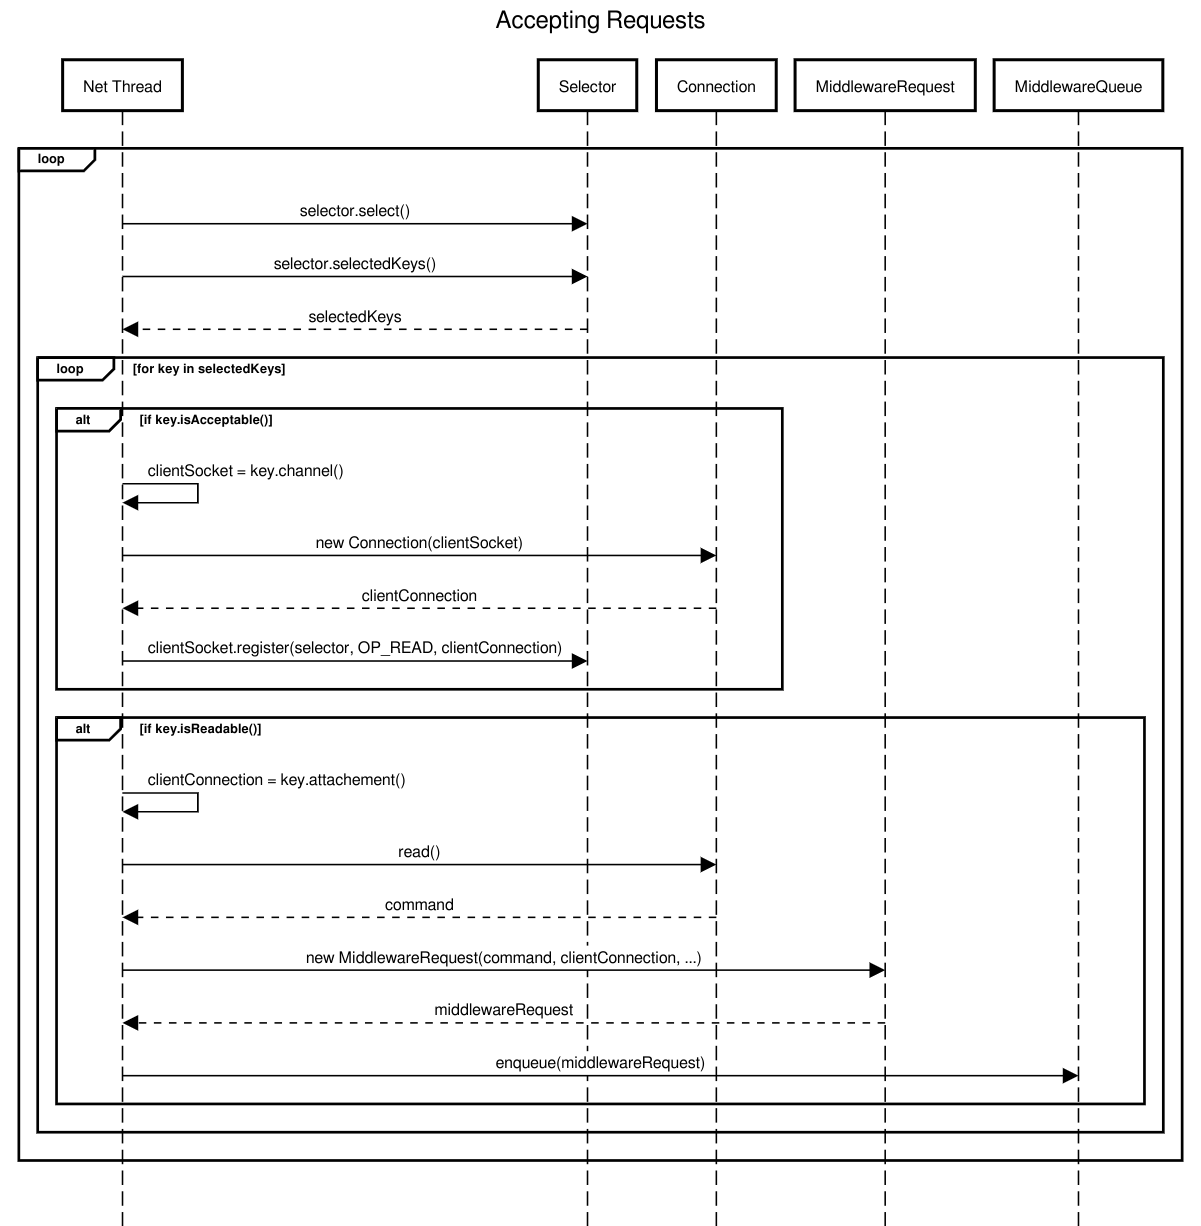
\includegraphics[width=\linewidth]{../illustrations/accepting_requests.png}
    \caption{Accepting new connections and requests}
    \label{fig:accepting_requests}
\end{figure}
%
\begin{figure}[H]
    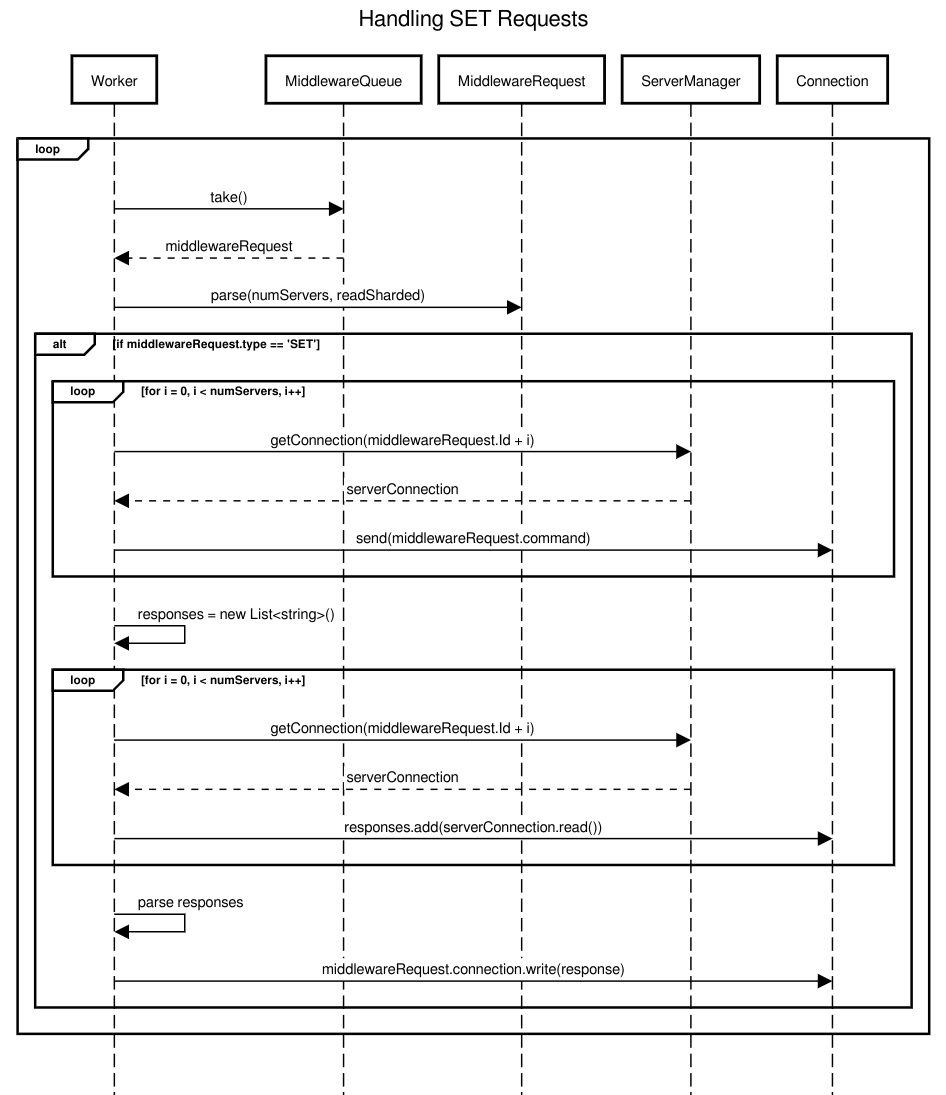
\includegraphics[width=\linewidth]{../illustrations/handling_set.png}
    \caption{Handling \texttt{SET} requests}
    \label{fig:handling_set}
\end{figure}
%
\begin{figure}[H]
    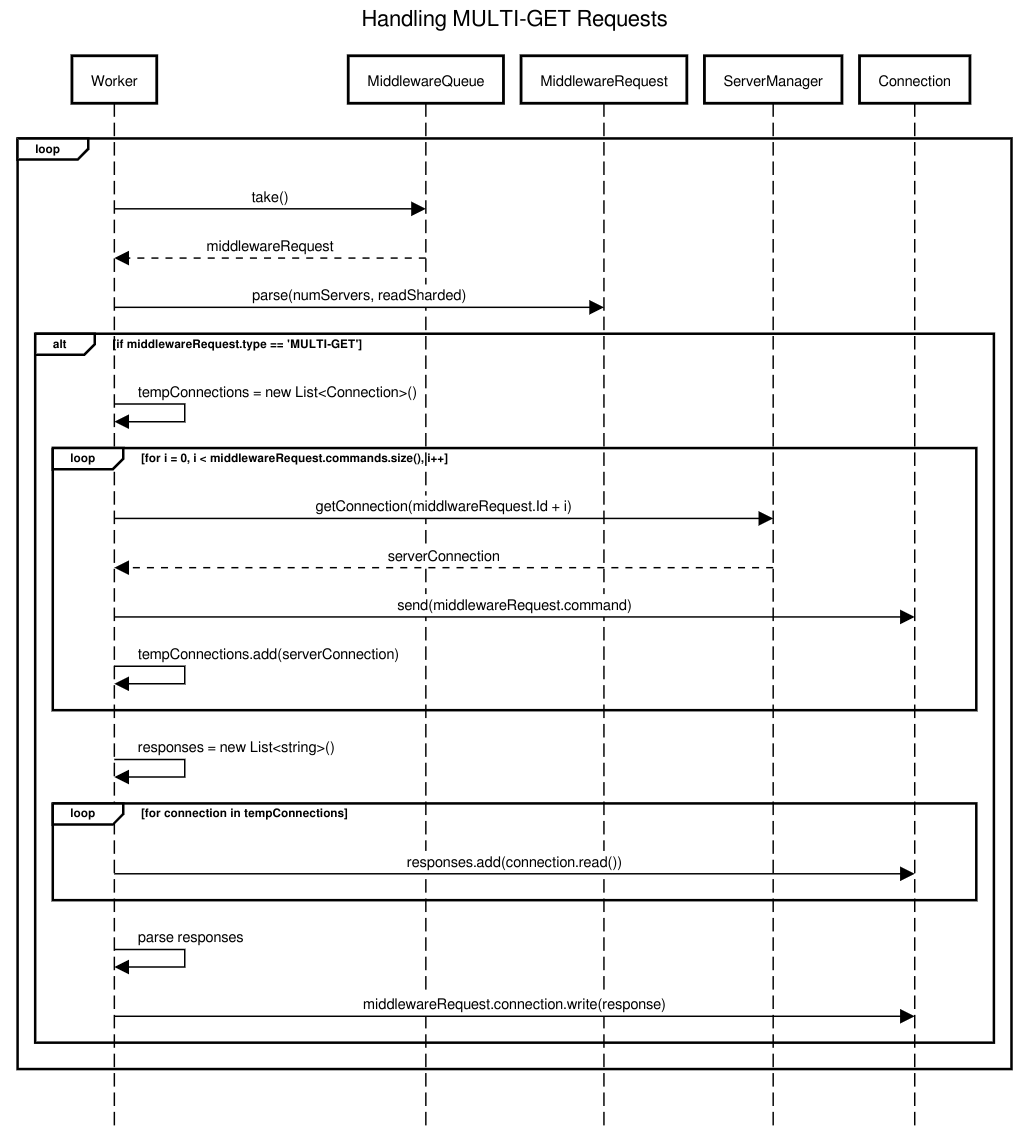
\includegraphics[width=\linewidth]{../illustrations/handling_mget.png}
    \caption{Handling \texttt{MULTI-GET} requests}
    \label{fig:handling_mget}
\end{figure}
%
\begin{figure}[H]
    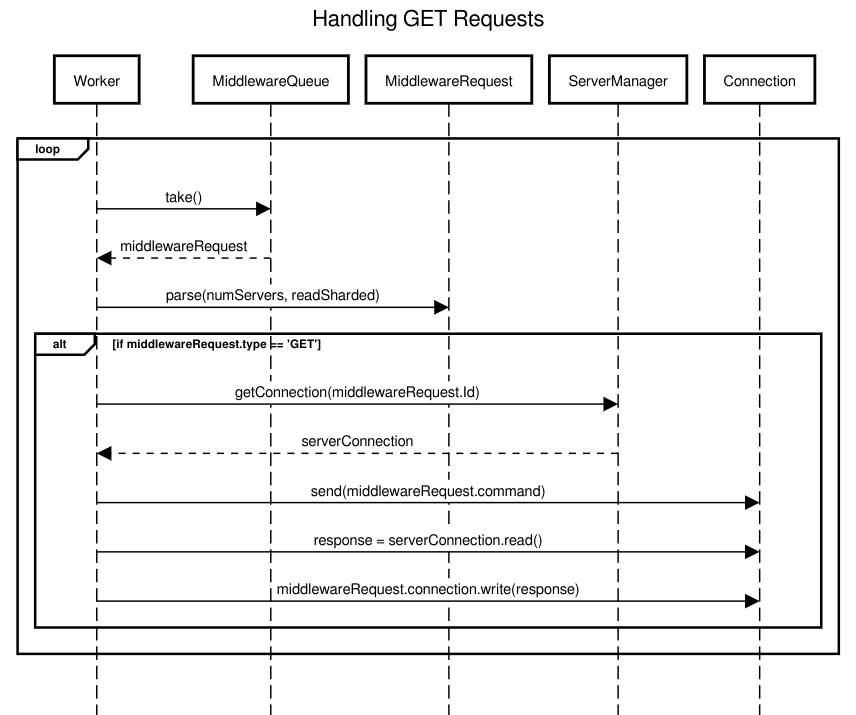
\includegraphics[width=\linewidth]{../illustrations/handling_get.png}
    \caption{Handling \texttt{GET} requests}
    \label{fig:handling_get}
\end{figure}
%
\subsection{Measurements}
%
Before getting into the analysis I want to lose a few words on the measurements and how they are handled.
%
\paragraph{No Middleware}
%
In this case we rely entirely on the output of \texttt{memtier\_benchmark}.
%
There we receive detailed numbers on number of requests and latency, however aggregated per one second intervals.
%
\paragraph{Middleware}
%
In this case we can use the detailed measurements from the middleware logs to produce the plots.
%
The measurements use \texttt{System.nanoTime()} in combination with \\ \texttt{System.currentTimeMillis()} to produce nanosecond Unix Timestamps.
%
We can compute the response time for each request and aggregate the average over all the requests.
%
When computing the average throughput we create a histogram based on the time a request was completed with the same number of bins as the duration of the experiment in seconds.
%
After that we sum these values over all middlewares and compute the average over the seconds the experiments was running.
%
All the plots use the 95\% percent confidence interval as an error measure.
%
\section{Baseline without Middleware (75 pts)}
%
\subsection{One Server}
%
\subsubsection{System Setup}
%
For this experiment we will use the following system setup:
%
\begin{itemize}
	\item 3 client machines with 1 memtier instance per machine. Each instance of memtier runs with 2 threads.
	\item No middlewares
	\item 1 memcached server
\end{itemize}
%
We vary the number of virtual clients per thread from 1 to 32.
%
\subsubsection{Objective}
%
The objective of this experiment is to find out how much load a single server can handle.
%
This means we will increase the number of virutal clients until the memcached server is the bottleneck of the system.
%
\subsubsection{Explanation}
%
\paragraph{Write-Only Workload}
%
\begin{figure}[H]
	\centering
    \begin{minipage}{0.5\textwidth}
        \centering
        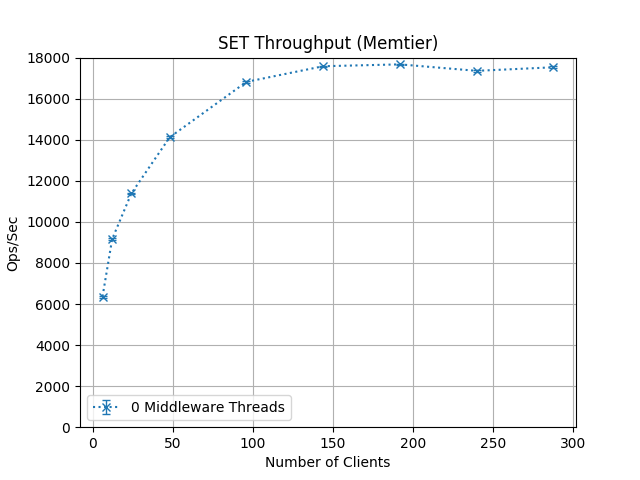
\includegraphics[width=\textwidth]{../illustrations/plots/1_1_one_server/1-0/memtier_set_tp_s.png}
        \caption{\texttt{SET} Throughput}
        \label{fig:one_server_set_tp}
    \end{minipage}\hfill
    \begin{minipage}{0.5\textwidth}
        \centering
        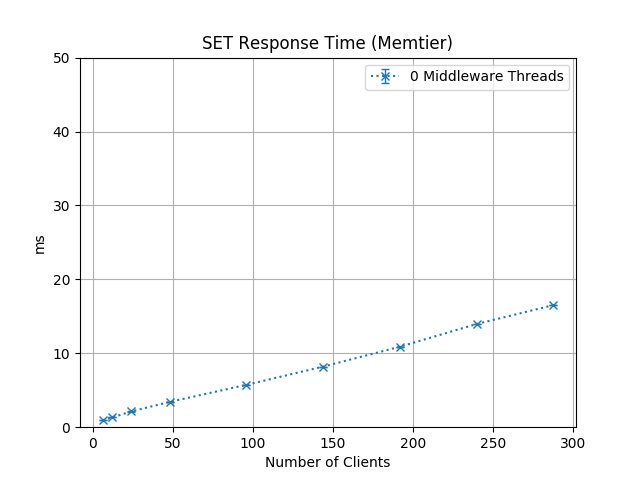
\includegraphics[width=\textwidth]{../illustrations/plots/1_1_one_server/1-0/memtier_set_rt_ms.png}
        \caption{\texttt{SET} Response Time}
        \label{fig:one_server_set_rt}
    \end{minipage}
\end{figure}
%
As mentioned in the objective we want to find out how much, in this case write requests, one memcached server can handle, i.e. how many clients do we need such that the server is saturated.
%
We can see that the server is saturated by two things:
%
\begin{itemize}
	\item The throughput of the system does not increase anymore when increasing the number of clients. We can determine that easily by if the throughput plot shows a flat line after some point.
	\item The response time increases linearly. In an ideal system the response time stays flat when the system is not saturated. However in practice a lot of factors can influence the response time, so it might be increasing in a undersaturated system. What we look for in the response time plot is a "knee" which shows an increase in the amount the response increases per new client. 
\end{itemize}
%
In general we will try to use the two conditions above to determine the point at which the system gets saturated.
%
\todo{interactive law check, maybe print a latex table when generating the plot with already filled in values for all experiments.}
%
As we can see in figure~\ref{fig:one_server_set_tp} we can achieve approximately 16000 ops/sec before the server is completely saturated, using 96 clients.
%
In figure~\ref{fig:one_server_set_rt} it is more difficult to identify the point at which the system is saturated. 
%
However we can see a small increase in the slope of the response time at 96 clients, which supports the claim done based on the throughput plot.
%
Oversaturation does not occur in this experiment.
%
Since this is the very first experiment we cannot yet compare it to much.
%
The take away message here is that one memcached server can handle up to approximately 16000 write ops/sec and is saturated when using 96 clients.
%
Also we conclude definitely that memcached is the bottleneck of the system in this configuration and using this specific workload.
%
\paragraph{Read-Only Workload}
%
\begin{figure}[H]
    \centering
    \begin{minipage}{0.5\textwidth}
        \centering
        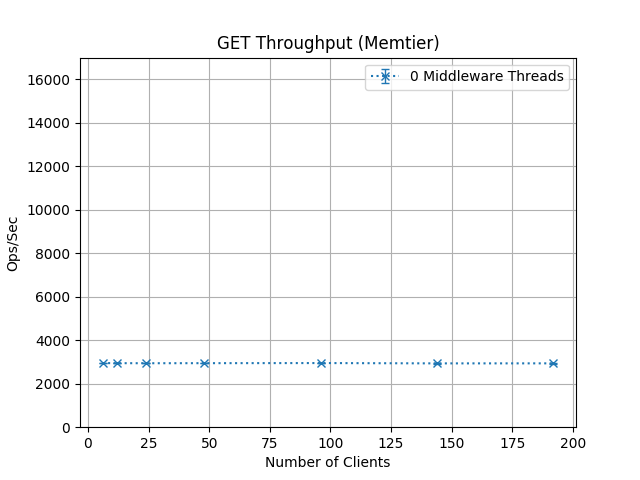
\includegraphics[width=\textwidth]{../illustrations/plots/1_1_one_server/0-1/memtier_get_tp_s.png}
        \caption{\texttt{GET} Throughput}
        \label{fig:one_server_get_tp}
    \end{minipage}\hfill
    \begin{minipage}{0.5\textwidth}
        \centering
        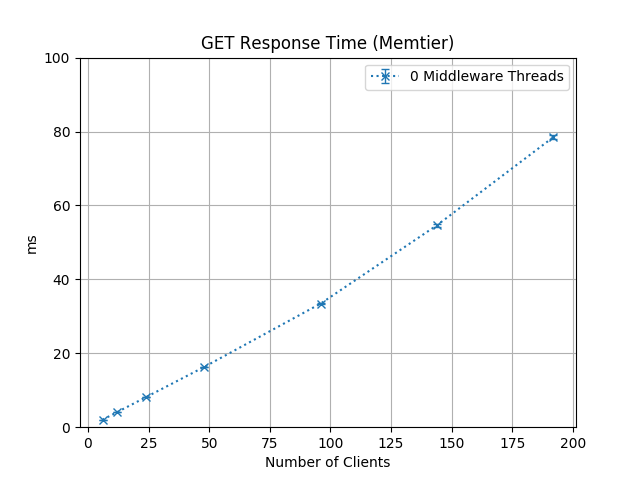
\includegraphics[width=\textwidth]{../illustrations/plots/1_1_one_server/0-1/memtier_get_rt_ms.png}
        \caption{\texttt{GET} Response Time}
        \label{fig:one_server_get_rt}
    \end{minipage}
\end{figure}
%
In figure~\ref{fig:one_server_get_tp} we see that the system can handle approximately 3000 read ops/sec.
%
As we have seen above the memcached server performs massively better for \texttt{SET} requests.
%
The reason for this is rather straight forward.
%
When handling \texttt{SET} requests the server can just store the record.
%
Usually this is done by hashing the key and storing the value in some sort of hash table, which is a operation that takes $O(1)$ time, since memcached stores all values in memory.
%
However when handling \texttt{GET} requests the server must hash the key, which is still done in constant time, but after hashing the server must actually retrieve the associated value from memory and send it to the client, which takes $O(s)$ time where $s$ is the size of the stored value.
%
The memcached server seems to be saturated even when using only 6 clients.
%
The saturation can is clearly depicted in figure~\ref{fig:one_server_get_tp}.
%
This hypothesis is also supported by the response time, we can see that from the start the response time increases linearly, without increasing the slope at some point during the experiment.
%
Oversaturation does not occur in this experiment even when using 192 virtual clients.
%
\\
%
Since we could not identify an undersaturated phase of the system we ran an additional experiment.
%
The setup was that we used only one load generating machine with only one instance of memtier running only one thread.
%
The virtual clients were varied from 1 to 8, since above we saw an saturation at 6 clients we would expect this experiment to reveal an undersaturated memcached server.
%
\begin{figure}[H]
    \centering
    \begin{minipage}{0.5\textwidth}
        \centering
        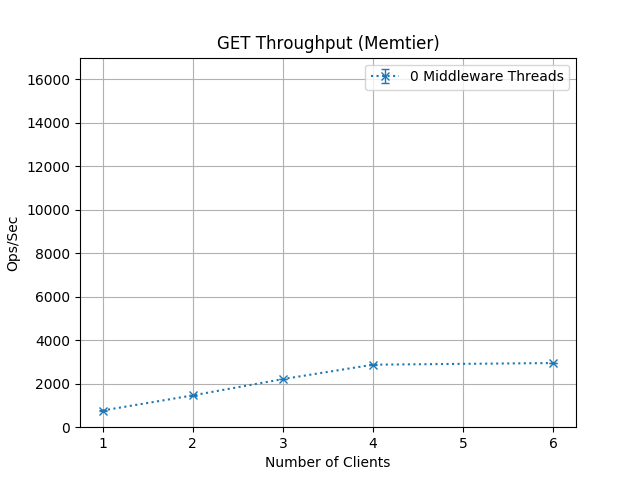
\includegraphics[width=\textwidth]{../illustrations/plots/1_1_1_one_server_reduced/0-1/memtier_get_tp_s.png}
        \caption{\texttt{GET} Throughput}
        \label{fig:one_server_reduced_get_tp}
    \end{minipage}\hfill
    \begin{minipage}{0.5\textwidth}
        \centering
        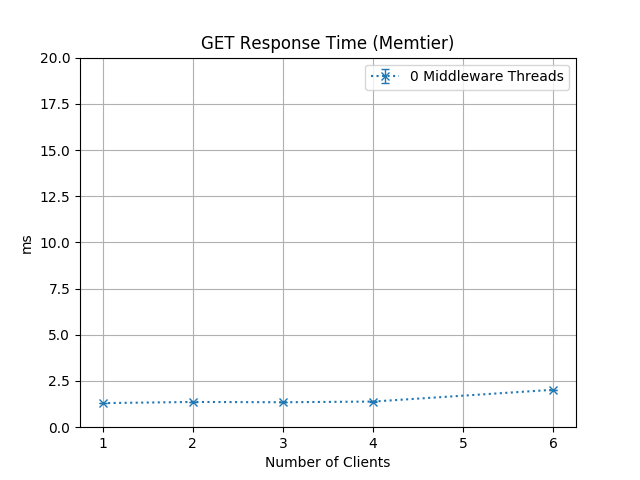
\includegraphics[width=\textwidth]{../illustrations/plots/1_1_1_one_server_reduced/0-1/memtier_get_rt_ms.png}
        \caption{\texttt{GET} Response Time}
        \label{fig:one_server_reduced_get_rt}
    \end{minipage}
\end{figure}
%
As we can see rather clearly in figure~\ref{fig:one_server_reduced_get_tp} the memcached server is already saturated using only 2 clients in total.
%
Also in figure~\ref{fig:one_server_reduced_get_rt} we can identify the response time starting to increase after two clients.
%
\subsection{Two Servers}
%
\subsubsection{System Setup}
%
For this experiment we will use the following system setup:
%
\begin{itemize}
	\item 1 client machines with 2 memtier instances per machine. Each instance of memtier runs with 1 threads.
	\item No middlewares
	\item 2 memcached servers
\end{itemize}
%
We vary the number of virtual clients per thread from 1 to 32.
%
\subsubsection{Objective}
%
In this experiment we turn to the clients.
%
The idea is to find out how much requests the clients can produce.
%
Assuming the clients will not be the bottleneck of the system we should be able to double the throughput from the previous experiments.
%
If the clients will be the bottleneck we expect the throughput of the system to be lower than in the previous section.
%
\subsubsection{Explanation}
%
\paragraph{Write-Only Workload}
%
\begin{figure}[H]
	\centering
    \begin{minipage}{0.5\textwidth}
        \centering
        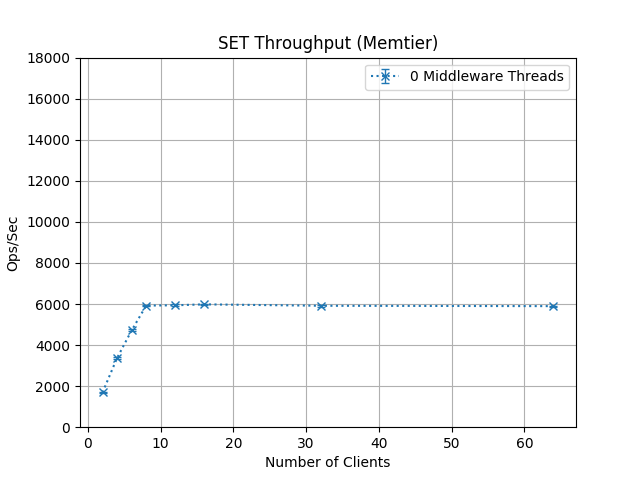
\includegraphics[width=\textwidth]{../illustrations/plots/1_2_two_servers/1-0/memtier_set_tp_s.png}
        \caption{\texttt{SET} Throughput}
        \label{fig:two_servers_set_tp}
    \end{minipage}\hfill
    \begin{minipage}{0.5\textwidth}
        \centering
        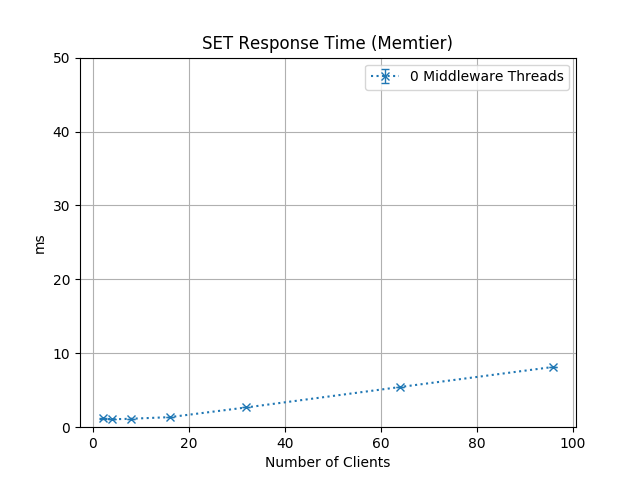
\includegraphics[width=\textwidth]{../illustrations/plots/1_2_two_servers/1-0/memtier_set_rt_ms.png}
        \caption{\texttt{SET} Response Time}
        \label{fig:two_servers_set_rt}
    \end{minipage}
\end{figure}
%
In these two plots we can see both conditions for a saturated phase very clearly.
%
After 16 clients the throughput does not increase at all anymore and reaches a maximum of approximately 6000 write ops/sec.
%
This can be supported by looking at the response time, where we can clearly see the "knee" in the plot after 16 clients.
%
From the previous section we know that one memcached server can handle approximately 16000 write ops/sec which means, since here we have 2 servers, if the servers were the bottleneck we should see double that number.
%
This would lead to the conclusion that the only other participant must be the bottleneck, namely memtier.
%
But in figure~\ref{fig:two_servers_set_rt} we can see that "knee" in the graph, indicating that the memcached server could be the bottleneck.
%
I still conclude that memtier is the bottleneck, since if we compare the absolute values with figure\ref{fig:one_server_set_rt} we quickly see that a saturated memcached server produces response times a lot higher than what we measured in this experiment.
%
An ideal server would show a constant response time, but comparing the roughly 9ms we measured here for 92 clients with the approximately 35ms measured with only one server, we can conclude that we are not dealing with saturated memcached servers here.
%
\paragraph{Read-Only Workload}
%
\begin{figure}[H]
	\centering
    \begin{minipage}{0.5\textwidth}
        \centering
        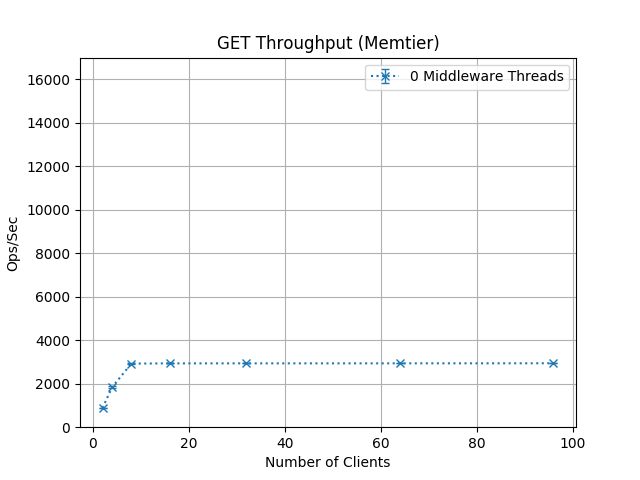
\includegraphics[width=\textwidth]{../illustrations/plots/1_2_two_servers/0-1/memtier_get_tp_s.png}
        \caption{\texttt{GET} Throughput}
        \label{fig:two_servers_get_tp}
    \end{minipage}\hfill
    \begin{minipage}{0.5\textwidth}
        \centering
        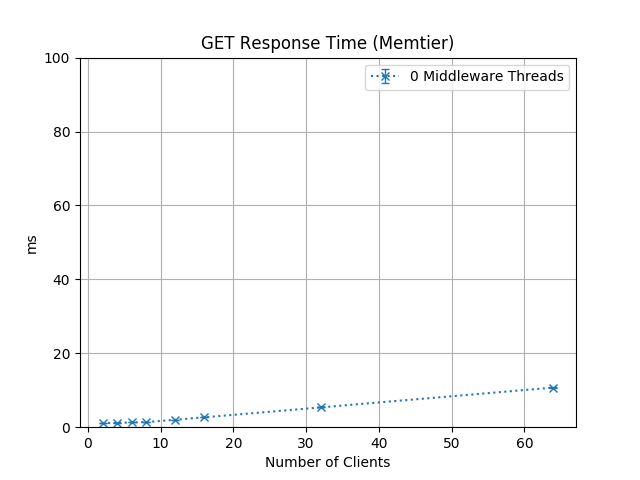
\includegraphics[width=\textwidth]{../illustrations/plots/1_2_two_servers/0-1/memtier_get_rt_ms.png}
        \caption{\texttt{GET} Response Time}
        \label{fig:two_servers_get_rt}
    \end{minipage}
\end{figure}
%
Again here we can clearly the the saturation of the system.
%
However the system is already saturated using only 8 clients in total.
%
This is not surprising since we know from before that \texttt{GET} requests are more expensive for the server than \texttt{SET} requests.
%
What is interesting however is that we can produce almost exactly the same amount of read operations per second than write operations. 
%
From this we conclude that the generation of the payload for \texttt{SET} requests produces a negligible overhead on the client machines.
%
However here it is not as clear cut as before that memtier is the bottleneck.
%
As we saw in figure~\ref{fig:one_server_get_tp} one server alone can handle approximately 3000 ops/sec, therefore we expect that two saturated memcached servers together can serve about 6000 ops/sec.
%
In figure~\ref{fig:two_servers_get_tp} we see that in this case we achieve approximately 6000 read ops/sec.
%
This is the exact value we expected from memcached, however it is also the maximum number of requests a client machine can produce.
%
Therefore it is difficult to say exaclty whether memtier or the memcached server are the bottleneck of this system.
%
When we look at figure~\ref{fig:two_servers_get_rt} we can see that after 8 clients there is an increase in slope, which would indicate that the servers are the bottleneck, since the response time should, in theory, stay constant when the system is undersaturated.
%
In this case it is really difficult to conclude with certainty whether the server or memtier is the bottleneck, in this case the components are matched together very well.
%
\subsection{Summary}

Based on the experiments above, fill out the following table:

\begin{center}
	{Maximum throughput of different VMs.}
	\begin{tabular}{|l|p{2cm}|p{2cm}|p{4cm}|}
		\hline                        & Read-only workload & Write-only workload & Configuration gives max. throughput \\ 
		\hline One memcached server   & 2875 (4 Clients)   & 15643 (96 Clients)  & Write-Only, 96 Clients       \\ 
		\hline One load generating VM & 5810 (8 Clients)  & 5920 (12 Clients)   & Read-Only, 12 Clients         \\ 
		\hline 
	\end{tabular}
\end{center}
%
When we look at the Read-only workload we can see that when we double the amount of servers from one to two the throughput also doubles. 
%
This indicates again that in the first experiment the server is the bottleneck.
%
Further we can see that one server is already saturated with 4 clients, whereas when using two servers we can handle up to 8 clients with approximately double the requests before being saturated, which again supports the conclusion that the server was the bottleneck in the first experiment.
%
\\
%
Looking at the Write-only workload it looks a bit different.
%
We can see that when using less client machines the throughput decreases drastically, even if we use two servers.
%
As mentioned before this indicates that a client machine cannot generate more load.
%
This is because the clients will likely reach their hardware limit at some point, the resources of one machine are shared by too many virtual clients.
%
\\
%
Important to mention is that the numbers above to not always correspond to the absolute maximum throughput observed during the experiments.
%
For example the Write-only workload recorded a maximum throughput of 15850 at 192 clients, however we know that the system was saturated already with 96 clients, therefore the maximum throughput at 192 has little meaning.
%
\\
%
Summarizing the sections up to now we have a few key take away messages:
%
\begin{itemize}
	\item One memcached server alone can handle a lot more \texttt{SET} requests than \texttt{GET} requests, more than 5 times as much.
	\item One memcached server alone can handle about 16000 \texttt{SET} ops/sec and approximately 3000 \texttt{GET} ops/sec
	\item One client machine alone can generate up to approximately 6000 ops/sec
	\item For one client it does not really matter if it is generating \texttt{GET} or \texttt{SET} requests, when measuring how much ops/sec can be produced.
\end{itemize}
%
The absolute numbers here should only be used as an approximate measure, even just restarting the VMs can produce different results. 
%
The idea is to get a sense on the relation between the different configurations and approximate numbers.
%
\section{Baseline with Middleware (90 pts)}
%
\subsection{One Middleware}
%
\subsubsection{System Setup}
%
For this experiment we will use the following system setup:
%
\begin{itemize}
	\item 3 client machines with 1 memtier instances per machine. Each instance of memtier runs with 2 threads.
	\item 1 middleware
	\item 1 memcached server
\end{itemize}
%
We vary the number of virtual clients per thread from 1 to 48.
%
\subsubsection{Objective}
%
Similar to the first experiment we want to find out how much load a single middleware can handle. 
%
Again we will increase the number of virtual clients until the middleware is the bottleneck of the system.
%
We assume for now that one memcached server is more performing than the middleware and therefore it should not be a problem that we only use one server.
%
We will see later if this assumption is justified.
%
\subsubsection{Explanation}
%
\paragraph{Write-Only Workload}
%
\begin{figure}[H]
	\centering
    \begin{minipage}{0.5\textwidth}
        \centering
        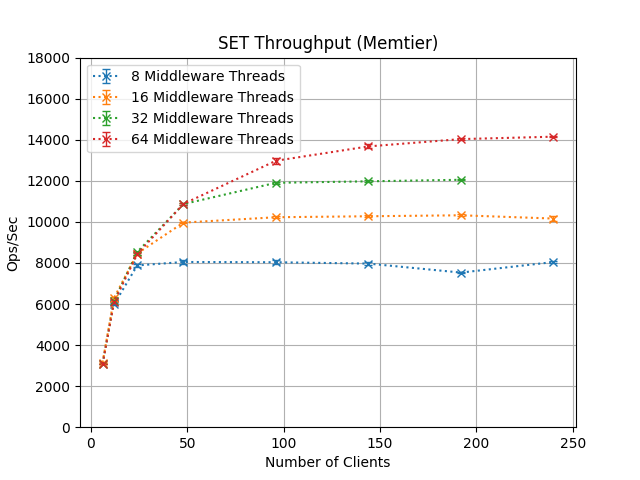
\includegraphics[width=\textwidth]{../illustrations/plots/2_1_one_middleware/1-0/memtier_set_tp_s.png}
        \caption{\texttt{SET} Throughput measured by memtier}
        \label{fig:one_middleware_set_tp_mt}
    \end{minipage}\hfill
    \begin{minipage}{0.5\textwidth}
        \centering
        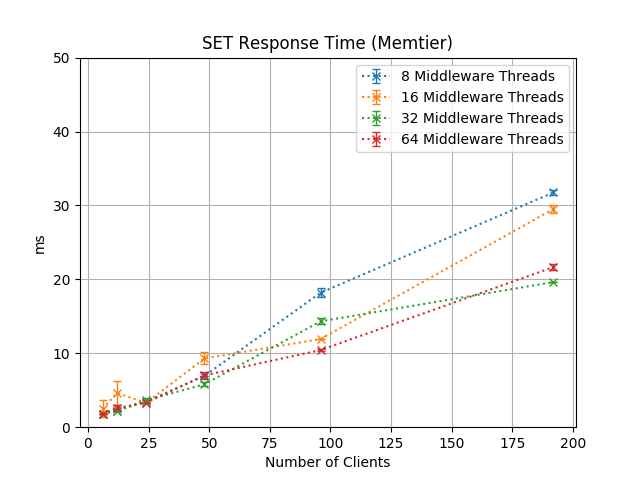
\includegraphics[width=\textwidth]{../illustrations/plots/2_1_one_middleware/1-0/memtier_set_rt_ms.png}
        \caption{\texttt{SET} Response Time measured by memtier}
        \label{fig:one_middleware_set_rt_mt}
    \end{minipage}
\end{figure}
%
\begin{figure}[H]
	\centering
    \begin{minipage}{0.5\textwidth}
        \centering
        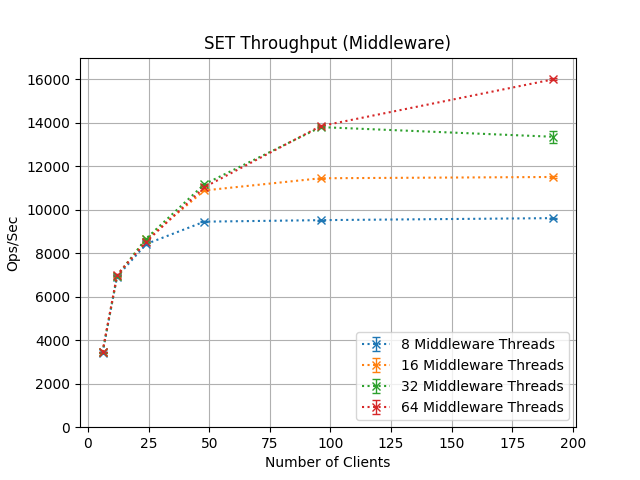
\includegraphics[width=\textwidth]{../illustrations/plots/2_2_two_middlewares/1-0/middleware_set_tp_s.png}
        \caption{\texttt{SET} Throughput measured by middleware}
        \label{fig:one_middleware_set_tp_mw}
    \end{minipage}\hfill
    \begin{minipage}{0.5\textwidth}
        \centering
        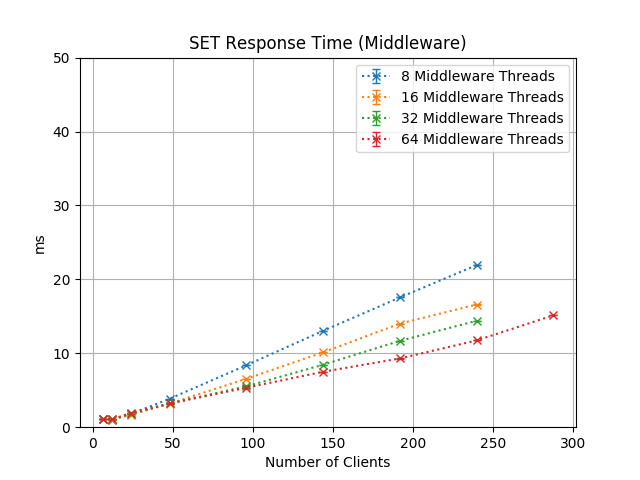
\includegraphics[width=\textwidth]{../illustrations/plots/2_2_two_middlewares/1-0/middleware_set_rt_ms.png}
        \caption{\texttt{SET} Response Time measured by middleware}
        \label{fig:one_middleware_set_rt_mw}
    \end{minipage}
\end{figure}
%
\paragraph{Read-Only Workload}
%
\begin{figure}[H]
	\centering
    \begin{minipage}{0.5\textwidth}
        \centering
        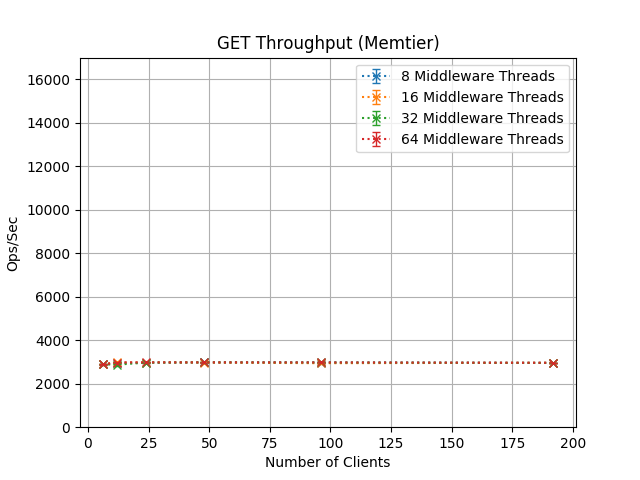
\includegraphics[width=\textwidth]{../illustrations/plots/2_1_one_middleware/0-1/memtier_get_tp_s.png}
        \caption{\texttt{SET} Throughput measured by memtier}
        \label{fig:one_middleware_set_tp_mt}
    \end{minipage}\hfill
    \begin{minipage}{0.5\textwidth}
        \centering
        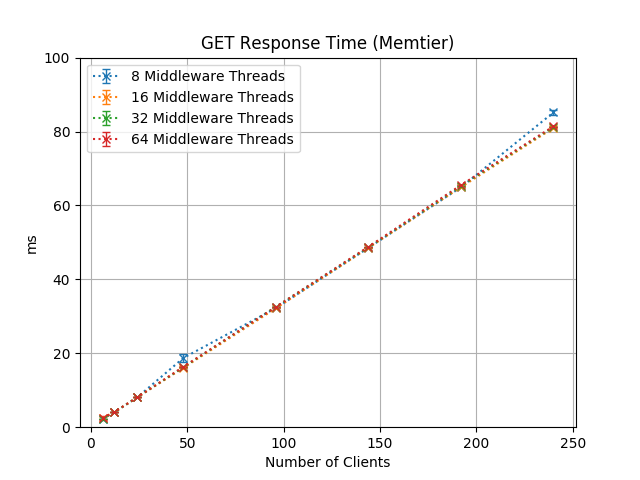
\includegraphics[width=\textwidth]{../illustrations/plots/2_1_one_middleware/0-1/memtier_get_rt_ms.png}
        \caption{\texttt{SET} Response Time measured by memtier}
        \label{fig:one_middleware_set_rt_mt}
    \end{minipage}
\end{figure}
%
\begin{figure}[H]
	\centering
    \begin{minipage}{0.5\textwidth}
        \centering
        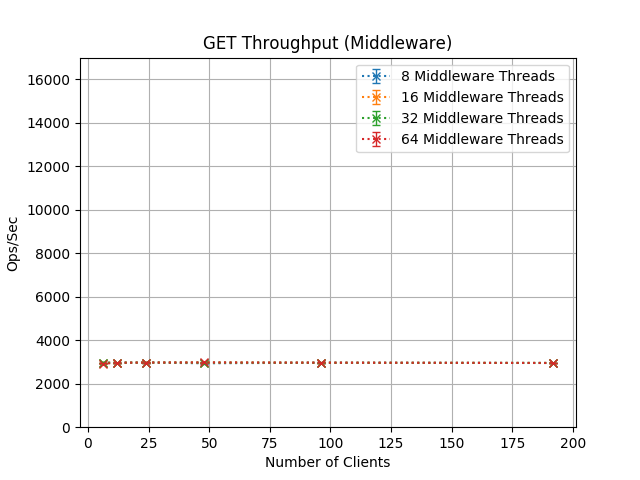
\includegraphics[width=\textwidth]{../illustrations/plots/2_2_two_middlewares/0-1/middleware_get_tp_s.png}
        \caption{\texttt{GET} Throughput measured by middleware}
        \label{fig:one_middleware_set_tp_mw}
    \end{minipage}\hfill
    \begin{minipage}{0.5\textwidth}
        \centering
        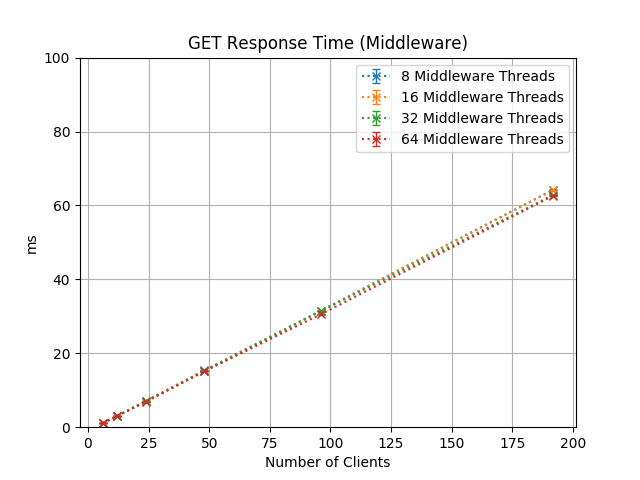
\includegraphics[width=\textwidth]{../illustrations/plots/2_2_two_middlewares/0-1/middleware_get_rt_ms.png}
        \caption{\texttt{GET} Response Time measured by middleware}
        \label{fig:one_middleware_set_rt_mw}
    \end{minipage}
\end{figure}



































\subsection{Two Middlewares}

Connect three load generator machines (two instances of memtier with CT=1) to two middlewares and use 1 memcached server. Run a read-only and a write-only workload with increasing number of clients (between 2 and 64) and measure response time \emph{both at the client and at the middleware}, and plot the throughput and response time as measured in the middleware.

Repeat this experiment for different number of worker threads inside the middleware: 8, 16, 32, 64.

\begin{center}
	\scriptsize{
		\begin{tabular}{|l|c|}
			\hline Number of servers                & 1                        \\ 
			\hline Number of client machines        & 3                        \\ 
			\hline Instances of memtier per machine & 2                        \\ 
			\hline Threads per memtier instance     & 1                        \\
			\hline Virtual clients per thread       & [1..32]                  \\ 
			\hline Workload                         & Write-only and Read-only \\
			\hline Multi-Get behavior               & N/A                      \\
			\hline Multi-Get size                   & N/A                      \\
			\hline Number of middlewares            & 2                        \\
			\hline Worker threads per middleware    & [8..64]                  \\
			\hline Repetitions                      & 3 or more (at least 1 minute each)                \\ 
			\hline 
		\end{tabular}
	} 
\end{center}

\subsubsection{Explanation}

Provide a detailed analysis of the results (e.g., bottleneck analysis, component utilizations, average queue lengths, system saturation). Add any additional figures and experiments that help you illustrate your point and support your claims.

\subsection{Summary}

Based on the experiments above, fill out the following table. For both of them use the numbers from a single experiment to fill out all lines. Miss rate represents the percentage of GET requests that return no data. Time in the queue refers to the time spent in the queue between the net-thread and the worker threads.


\begin{center}
	{Maximum throughput for one middleware.}
	\begin{tabular}{|l|p{2cm}|p{2cm}|p{2cm}|p{2cm}|}
		\hline                                & Throughput & Response time & Average time in queue & Miss rate \\ 
		\hline Reads: Measured on middleware  &            &               &                       &           \\ 
		\hline Reads: Measured on clients     &            &               & n/a                   &           \\ 
		\hline Writes: Measured on middleware &            &               &                       & n/a       \\ 
		\hline Writes: Measured on clients    &            &               & n/a                   & n/a       \\ 
		\hline 
	\end{tabular}
\end{center}

\begin{center}
	{Maximum throughput for two middlewares.}
	\begin{tabular}{|l|p{2cm}|p{2cm}|p{2cm}|p{2cm}|}
		\hline                                & Throughput & Response time & Average time in queue & Miss rate \\ 
		\hline Reads: Measured on middleware  &            &               &                       &           \\ 
		\hline Reads: Measured on clients     &            &               & n/a                   &           \\ 
		\hline Writes: Measured on middleware &            &               &                       & n/a       \\ 
		\hline Writes: Measured on clients    &            &               & n/a                   & n/a       \\ 
		\hline 
	\end{tabular}
\end{center}

Based on the data provided in these tables, write at least two paragraphs summarizing your findings about the performance of the middleware in the baseline experiments.

\section{Throughput for Writes (90 pts)}

\subsection{Full System}

Connect three load generating VMs to two middlewares and three memchached servers. Run a write-only experiment. 
You need to plot throughput and response time measured on the middleware as a function of number of clients. The measurements have to be performed for 8, 16, 32 and 64 worker threads inside each middleware.

\begin{center}
	\scriptsize{
		\begin{tabular}{|l|c|}
			\hline Number of servers                & 3          \\ 
			\hline Number of client machines        & 3          \\ 
			\hline Instances of memtier per machine & 2          \\ 
			\hline Threads per memtier instance     & 1          \\
			\hline Virtual clients per thread       & [1..32]    \\ 
			\hline Workload                         & Write-only \\
			\hline Multi-Get behavior               & N/A        \\
			\hline Multi-Get size                   & N/A        \\
			\hline Number of middlewares            & 2          \\
			\hline Worker threads per middleware    & [8..64]    \\
			\hline Repetitions                      & 3 or more (at least 1 minute each)  \\ 
			\hline 
		\end{tabular}
	} 
\end{center}

\subsubsection{Explanation}

Provide a detailed analysis of the results (e.g., bottleneck analysis, component utilizations, average queue lengths, system saturation). Add any additional figures and experiments that help you illustrate your point and support your claims.

\subsection{Summary}

Based on the experiments above, fill out the following table with the data corresponding to the maximum throughput point for all four worker-thread scenarios.

\begin{center}
	{Maximum throughput for the full system}
	\begin{tabular}{|l|p{1.5cm}|p{1.5cm}|p{1.5cm}|p{1.5cm}|}
		\hline                                            & WT=8 & WT=16 & WT=32 & WT=64 \\ 
		\hline Throughput (Middleware)                    &      &       &       &       \\ 
		\hline Throughput (Derived from MW response time) &      &       &       &       \\ 
		\hline Throughput (Client)                        &      &       &       &       \\ 
		\hline Average time in queue                      &      &       &       &       \\ 
		\hline Average length of queue                    &      &       &       &       \\ 
		\hline Average time waiting for memcached         &      &       &       &       \\ 
		\hline 
	\end{tabular}
\end{center}

Based on the data provided in these tables, draw conclusions on the state of your system for a variable number of worker threads.

\section{Gets and Multi-gets (90 pts)}

For this set of experiments you will use three load generating machines, two middlewares and three memcached servers. Each memtier instance should have 2 virtual clients in total and the number of middleware worker threads is 64, or the one that provides the highest throughput in your system (whichever number of threads is smaller).

For multi-GET workloads, use the \texttt{--ratio} parameter to specify the exact ratio between SETs and GETs. You will have to measure response time on the client as a function of multi-get size, with and without sharding on the middlewares.

\subsection{Sharded Case}

Run multi-gets with 1, 3, 6 and 9 keys (memtier configuration) with sharding enabled (multi-gets are broken up into smaller multi-gets and spread across servers). Plot average response time as measured on the client, as well as the 25th, 50th, 75th, 90th and 99th percentiles.

\begin{center}
	\scriptsize{
		\begin{tabular}{|l|c|}
			\hline Number of servers                & 3                       \\ 
			\hline Number of client machines        & 3                       \\ 
			\hline Instances of memtier per machine & 2                       \\ 
			\hline Threads per memtier instance     & 1                       \\
			\hline Virtual clients per thread       & 2     		            \\ 
			\hline Workload                         & ratio=1:$<$Multi-Get size$>$             \\
			\hline Multi-Get behavior               & Sharded                 \\
			\hline Multi-Get size                   & [1..9]                  \\
			\hline Number of middlewares            & 2                       \\
			\hline Worker threads per middleware    & max. throughput config. \\
			\hline Repetitions                      & 3 or more (at least 1 minute each)               \\ 
			\hline 
		\end{tabular}
	} 
\end{center}

\subsubsection{Explanation}

Provide a detailed analysis of the results (e.g., bottleneck analysis, component utilizations, average queue lengths, system saturation). Add any additional figures and experiments that help you illustrate your point and support your claims.

\subsection{Non-sharded Case}

Run multi-gets with 1, 3, 6 and 9 keys (memtier configuration) with sharding disabled. Plot average response time as measured on the client, as well as the 25th, 50th, 75th, 90th and 99th percentiles.

\begin{center}
	\scriptsize{
		\begin{tabular}{|l|c|}
			\hline Number of servers                & 3                       \\ 
			\hline Number of client machines        & 3                       \\ 
			\hline Instances of memtier per machine & 2                       \\ 
			\hline Threads per memtier instance     & 1                       \\
			\hline Virtual clients per thread       & 2                		 \\ 
			\hline Workload                         & ratio=1:$<$Multi-Get size$>$              \\
			\hline Multi-Get behavior               & Non-Sharded             \\
			\hline Multi-Get size                   & [1..9]                  \\
			\hline Number of middlewares            & 2                       \\
			\hline Worker threads per middleware    & max. throughput config. \\
			\hline Repetitions                      & 3 or more (at least 1 minute each)               \\ 
			\hline 
		\end{tabular}
	} 
\end{center}

\subsubsection{Explanation}

Provide a detailed analysis of the results (e.g., bottleneck analysis, component utilizations, average queue lengths, system saturation). Add any additional figures and experiments that help you illustrate your point and support your claims.

\subsection{Histogram}

For the case with 6 keys inside the multi-get, display four histograms representing the sharded and non-sharded response time distribution, both as measured on the client, and inside the middleware. Choose the bucket size in the same way for all four, and such that there are at least 10 buckets on each of the graphs.

\subsection{Summary}

Provide a detailed comparison of the sharded and non-shareded modes. For which multi-GET size is sharding the preferred option? Provide a detailed analysis of your system. Add any additional figures and experiments that help you illustrate your point and support your claims.

\section{2K Analysis (90 pts)}

For 3 client machines (with 64 total virtual clients per client VM) measure the throughput and response time of your system in a 2k experiment with repetitions. All GET operations have a single key. Investigate the following parameters:

\begin{itemize}
		
	\item Memcached servers: 1 and 3
	\item Middlewares: 1 and 2
	\item Worker threads per MW: 8 and 32
	      	      
\end{itemize}

Repeat the experiment for (a)~a write-only and (b)~a read-only workload.
For each of the two workloads, what is the impact of these parameters on throughput, respectively response time?

\begin{center}
	\scriptsize{
		\begin{tabular}{|l|c|}
			\hline Number of servers                & 1 and 3                                     \\ 
			\hline Number of client machines        & 3                                           \\ 
			\hline Instances of memtier per machine & 1 (1 middleware) or 2 (2 middlewares) \\ 
			\hline Threads per memtier instance     & 2 (1 middleware) or 1 (2 middlewares)   \\
			\hline Virtual clients per thread       &  32                                     \\ 
			\hline Workload                         & Write-only and Read-only\\
			\hline Multi-Get behavior               & N/A                                         \\
			\hline Multi-Get size                   & N/A                                         \\
			\hline Number of middlewares            & 1 and 2                                     \\
			\hline Worker threads per middleware    & 8 and 32                                    \\
			\hline Repetitions                      & 3 or more (at least 1 minute each)                                   \\ 
			\hline 
		\end{tabular}
	} 
\end{center}

\section{Queuing Model (90 pts)}

Note that for queuing models it is enough to use the experimental results from the previous sections. It is, however, possible that the numbers you need are not only the ones in the figures we asked for, but also the internal measurements that you have obtained through instrumentation of your middleware.

\subsection{M/M/1}

Build queuing model based on Section 4 (write-only throughput) for each worker-thread configuration of the middleware. Use one M/M/1 queue to model your entire system. Motivate your choice of input parameters to the model. Explain for which experiments the predictions of the model match and for which they do not.

\subsection{M/M/m}

Build an M/M/m model based on Section 4, where each middleware worker thread is represented as one service.  Motivate your choice of input parameters to the model. Explain for which experiments the predictions of the model match and for which they do not.

\subsection{Network of Queues}

Based on Section 3, build a network of queues which simulates your system. Motivate the design of your network of queues and relate it wherever possible to a component of your system. Motivate your choice of input parameters for the different queues inside the network. Perform a detailed analysis of the utilization of each component and clearly state what the bottleneck of your system is. Explain for which experiments the predictions of the model match and for which they do not.

\end{document}

